\chapter{全景漫游的交互模型}
全景漫游中的用户交互属于典型的多通道交互,根据前文所列举的关于人的意识的相关理论可知,人在面对多通道输入的刺激时,会或主动或被动地选择一种进行注意。如果这些刺激可以达到被人记忆并在需要时主动唤起的效果,那有可能在多通道输入中自动加工处理,减少对人的脑力资源的占用。同时,经过良好规划的交互模型也能避免用户出错的概率,提高网络资源的利用率,降低后台服务器程序处理的负担。

基于上述假设,尝试通过认知理论对全景漫游中设备端交互、菜单交互和场景交互,分别构建交互模型。以期通过多种形式展现信息,达到更高效表达场景的意图,结合人与设备的关系切实提升用户操作体验。

\section{设备交互}
交互从人发出的信息至被设备捕获转换为数字信号是一个明显的“编码/解码”的过程。人的动作相当于人通过分析相关信息,并试图理解机器的运作模式,认识到自己所需表达的信息,最后发出了一个按照“所认为机器能够理解的方式”进行编码的“信号”。而设备则是处在各种信息的海洋中,一刻不歇地从外界收集信息,当成功捕获到一个匹配其预设规律的“信号”时,通过确定的解码方式,还原出人最初想表达的信息。

\subsection{信息流与反馈等待}
设备无时无刻不在等待着用户的信息输入,而用户的输入是多通道的,在不同的通道上都会捕获到用户的输入流。多输入流经过处理后在主信息流上合并成一条输入流,由设备程序进行集中处理。如图\ref{fig:reactive}。

\begin{figure}[htp]
\centering
\fbox{
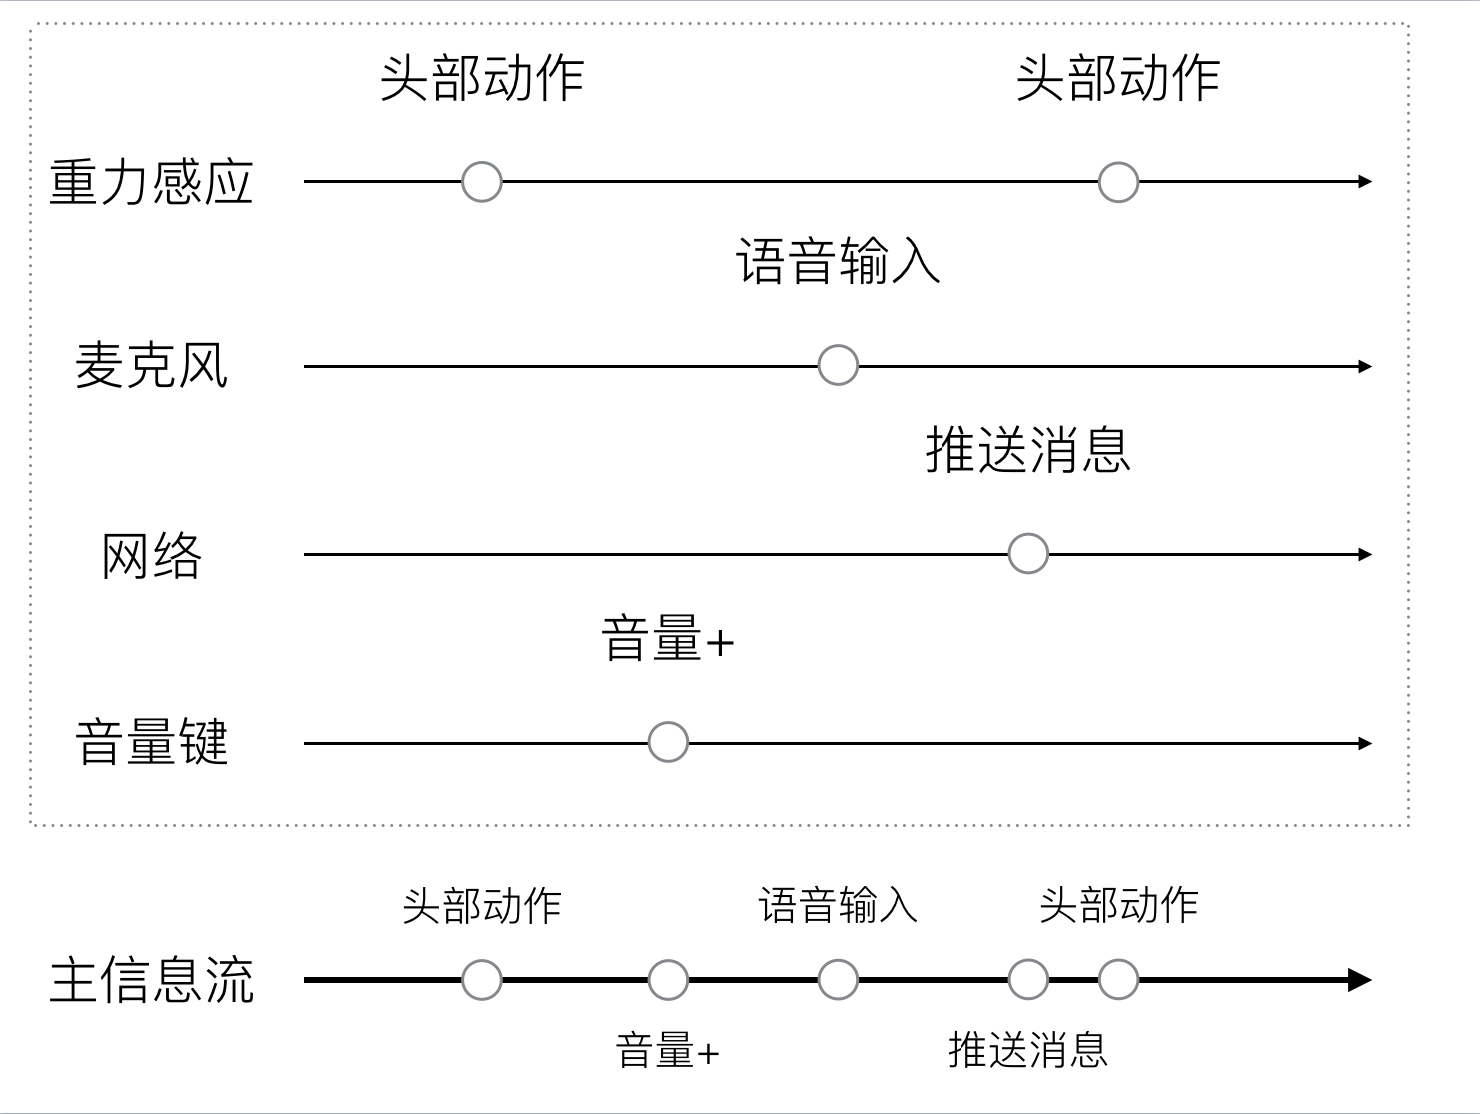
\includegraphics[width=.5\textwidth]{reactive}
}
\caption{信息流}
\label{fig:reactive}
\end{figure}

但常见的场景是,交互行为的发生与处理完成得到反馈并不是即时的,而要经过一定的时间,其等待时间因网络延迟或设备响应而不一。这时用户等待的过程就会形成一阵交互效果上的“盲区”,也就是常见的“设备无响应”状态,如图\ref{fig:stream}	。“设备无响应”情形在一般设备上出现并不会造成过大的后果,但是在全景漫游中用户的视野处在封闭的空间中,长时间得不到合理反馈易造成用户心理恐慌,是需要通过设计极力避免的情形。

\begin{figure}[htp]
\centering
\fbox{
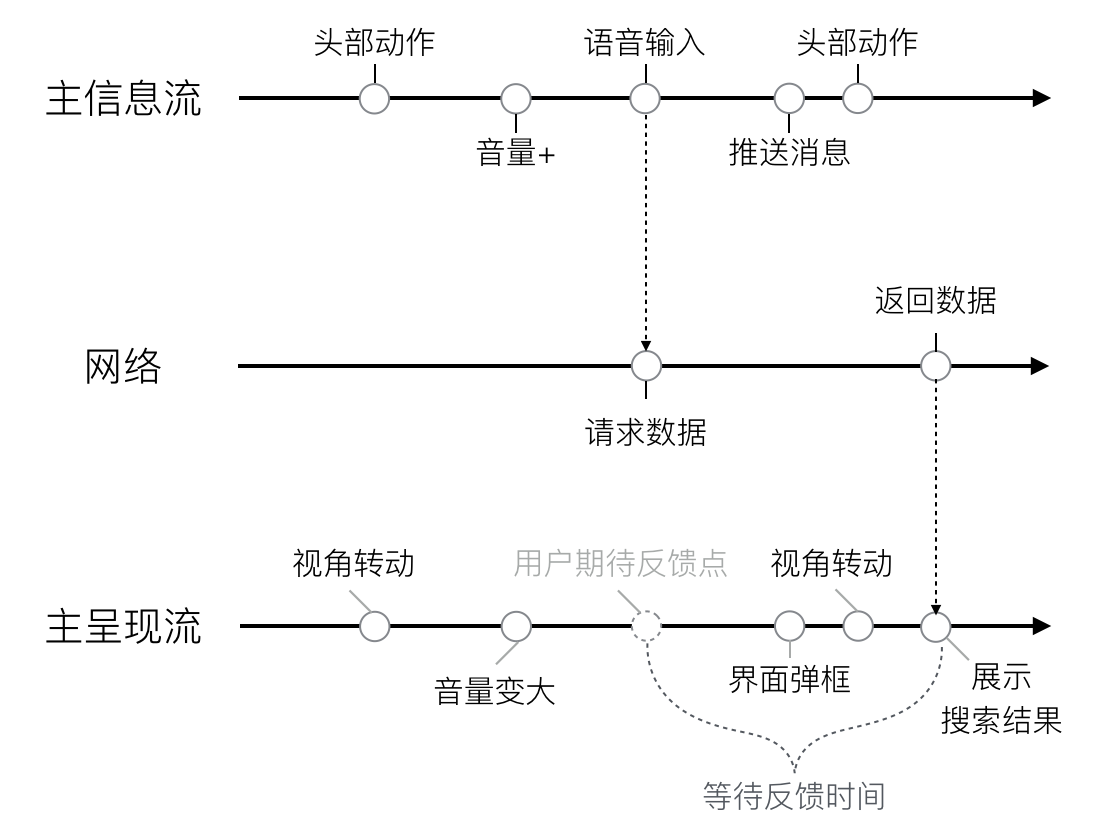
\includegraphics[width=.5\textwidth]{stream}
}
\caption{交互中因其他元素造成的等待}
\label{fig:stream}
\end{figure}

即时反馈信息是最理想的方案,但现实情况必须对此作出解释以避免用户等待无反馈而产生迷茫情绪。常见的方案是对用户的输入做出即时反馈,当反馈不能即时给到时给出等待反馈的提示。前文所提到的通过注视(gaze)一定时间而做出确定选择的过程就是一种非即时的操作,在等待确认完成过程中通过一些标示告知用户:此处正在等待完成的行为是什么,预计完成的时间是多少等。

\subsection{信息修正}
信息流的出现帮助解决了信息加工过程中信息传达时间不一致的问题,但用户有可能得到的信息不准确或是很模糊,需要用户去判断信息是否符合预期,在无法判断信息的有效性时,如果能够提供给用户一个可以自我纠正的语境,将有利于用户自己辨别信息\endnote{路璐,田丰,戴国忠,王宏安. 融合触、听、视觉的多通道认知和交互模型[J]. 计算机辅助设计与图形学学报,2014,(04):654-661.}。

例如,在导航过程中提供给给用户当前朝向与正确方向的箭头图示,用户会尝试向左或向右转向,当向左转时会发现偏离变大,而向右转时会发现偏离变小,用户自然会选择向右转以回到正确方向上去,如图\ref{fig:correct}。

\begin{figure}[htp]
\centering
\fbox{
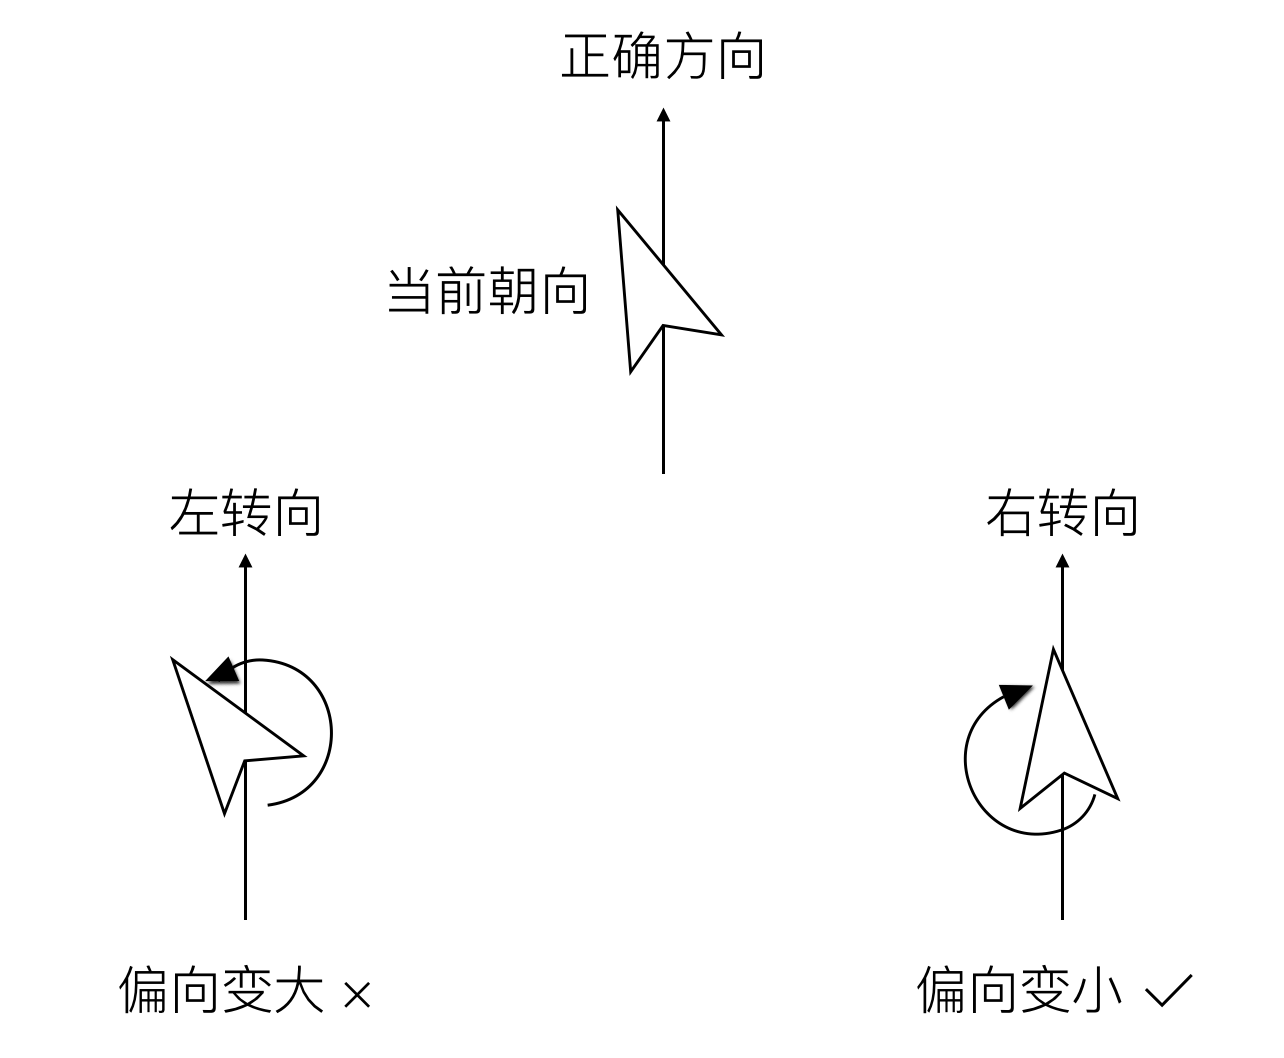
\includegraphics[width=.5\textwidth]{correct}
}
\caption{自我修正的交互行为}
\label{fig:correct}
\end{figure}

在全景漫游中与设备进行多通道交互是可行且必要的,人的感官可以从不同通道间获取信息,使人获得的信息更为全面。更为关键的是多通道信息往往能够起到互补的作用,使得信息交互的鲁棒性大大提高,也使用户对于系统和环境的适应性得到了提升。而全景漫游因与普通的设备交互有所不同,故应加强信息流的建立,避免用户无谓的等待,提高交互的流畅性。而在交互的结果上注重信息的可修正性,帮助用户通过自我反馈建立准确有效的信息流。

\section{导航交互}
全景漫游中导航功能的重要性不言而喻,但场景中元素的可识别要求又限制了导航功能的复杂度。导航应符合用户对信息整合的需求,而又对场景内容起烘托作用。由前一章信息架构的组织形式可知,导航应包括自顶向下、自底向上、不可见联结这三种基本信息组织形式,它们分别体现为导航层级的上下文感知、单个内容增强信息展示和多任务切换。

\subsection{上下文感知}
上下文是指当前环境中区别于当前本体的因素。上下文按与用户关系可简单分为主动上下文和被动上下文两种。主动上下文指环境中可以直接改变系统行为的状态或变量。被动上下文指那些虽不能直接产生作用但可引起用户兴趣继而通过用户改变系统行为的状态或变量\endnote{张磊. 上下文感知在导游系统中的应用[A]. 中国计算机学会、中国图象图形学学会、ACM SIGCHI中国分会、清华大学计算机科学与技术系.第一届建立和谐人机环境联合学术会议(HHME2005)论文集[C].中国计算机学会、中国图象图形学学会、ACM SIGCHI中国分会、清华大学计算机科学与技术系:,2005:4.}。上下文感知是指计算实体能够根据上下文环境的变化及时调整自身行为,使用户从信息的管理和输入中解放出来,专注于要执行任务的本身\endnote{王守芳, 金浩, 魏鲲,等. 上下文感知综述[C]// 建立和谐人机环境联合学术会议. 2005.}。

上下文感知的作用非常重要,没有上下文用户很难预计进行操作时即将发生的变化,容易在使用过程产生困惑。网页等在通过列表批量展示内容时都会同时展示该内容的多项信息,包括名称、录入时间、信息量等(可能因内容类型不同而信息名称有所差异)。例如商城类网页会展示商品的名称、产地、出厂时间等,这些信息就是上下文。通过阅读理解相关信息,用户可以在不打开具体页面的情况下对相应项目得到一个基本的认识。

上下文感知发生在上下文环境的改变过程中,具体表现为上下文语境的重构,即移除不再相关的组件,添加新的相关组件,同时改变组件间的联系等\endnote{李玲玲,高新. 基于上下文感知的移动计算应用[J]. 软件导刊,2011,(06):17-18.
}。

例如,在前文所提出的列表展示内容的页面中,当用户切换列表界面时,界面上标签的语义发生了变化,如图\ref{fig:context}。图中上半部分为分类的菜单,下半部分为某一分类的更多页面。上半部分中三个标签分别是不同的分类,而下半部分的三个标签则是针对同意分类的三种不同筛选方式。虽然两者形式上类似,但标签的语义截然不同。

\begin{figure}[htp]
\centering
\fbox{
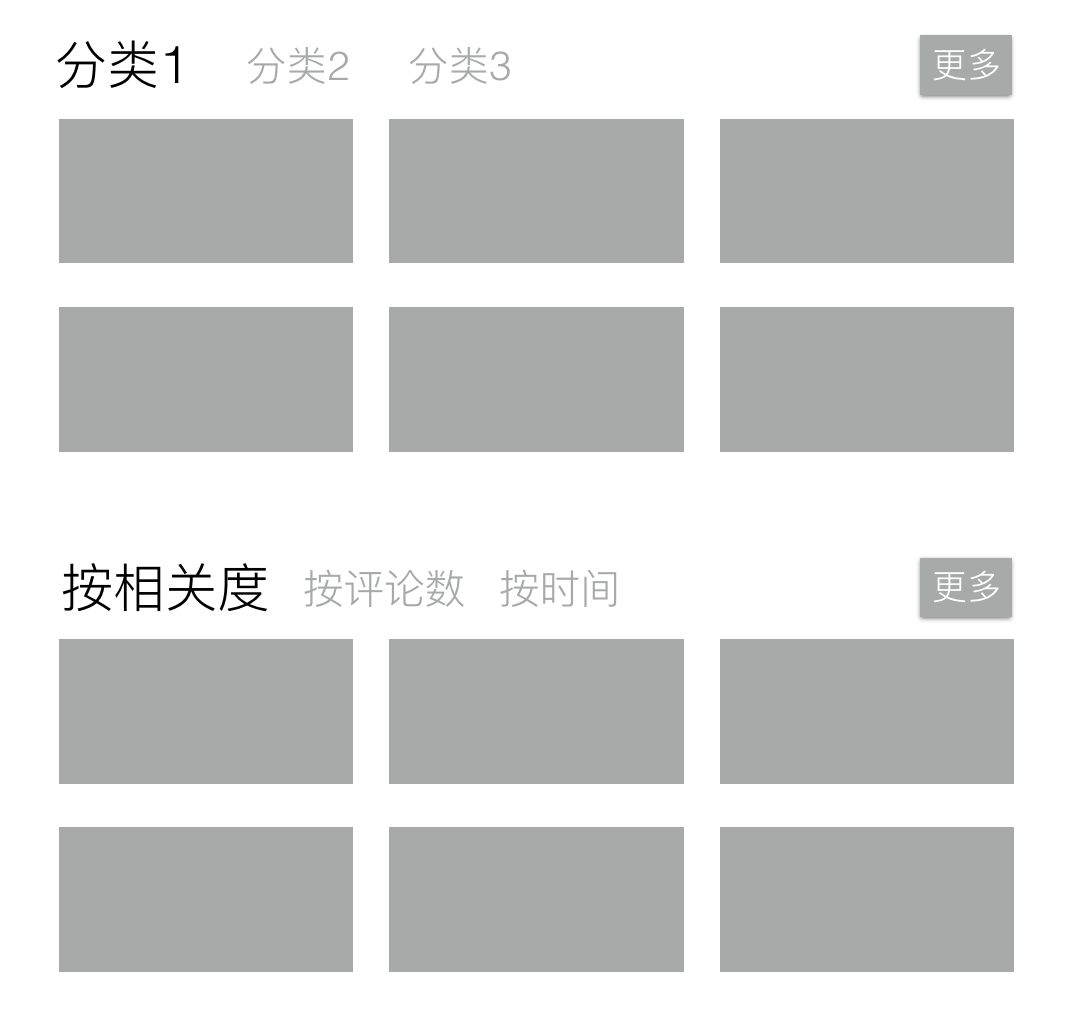
\includegraphics[width=.5\textwidth]{context}
}
\caption{上下文语境的重构}
\label{fig:context}
\end{figure}

\begin{table}[htbp]
\centering
\caption{分类菜单和单个类别菜单的语义}
\vskip 5pt
\begin{tabular}{lll}
\toprule
栏目 & 分类菜单 & 单个类别菜单 \\
\midrule
数据集合 & 不同 & 相同 \\
切换方式  & 点击标签 & 点击标签 \\
标签意义 & 集合代称 & 筛选依据 \\
\bottomrule
\end{tabular}
\label{tab:collection}
\end{table}

在上下文语境的重构过程中,语义的变化如表\ref{tab:collection}。表中可知,用户在语境切换后操作方式没有变化,依旧为点击标签,但单个标签的意义和数据的集合都发生了改变。这种情况下就容易造成上下文环境的语义混淆,需要直观且清晰地提示用户场景的语境已经发生变化,并标注上可供用户理解当前上下文环境的关键信息(如当前栏目的标示等)。

如图\ref{fig:tab},在 PC 端网页中,常用的标注语境的方式是一种“面包屑导航”,将从首页至当前页面所有途径的页面名称罗列出来。而在移动端设备上,因屏幕宽度上有限制,常用的做法是在顶部功能栏正中标注出当前栏目名称。而在全景漫游中,因界面不一定限制于二维空间内,故可以采用按深度排列的界面,以标示用户途径的界面。用户在切换界面时,同时可以看到曾经访问过的页面的一部分,容易理解该页面是由前一个页面中的部分扩展而来,对整体信息架构也会产生一定的了解。

\begin{figure}[htp]
\centering
\fbox{
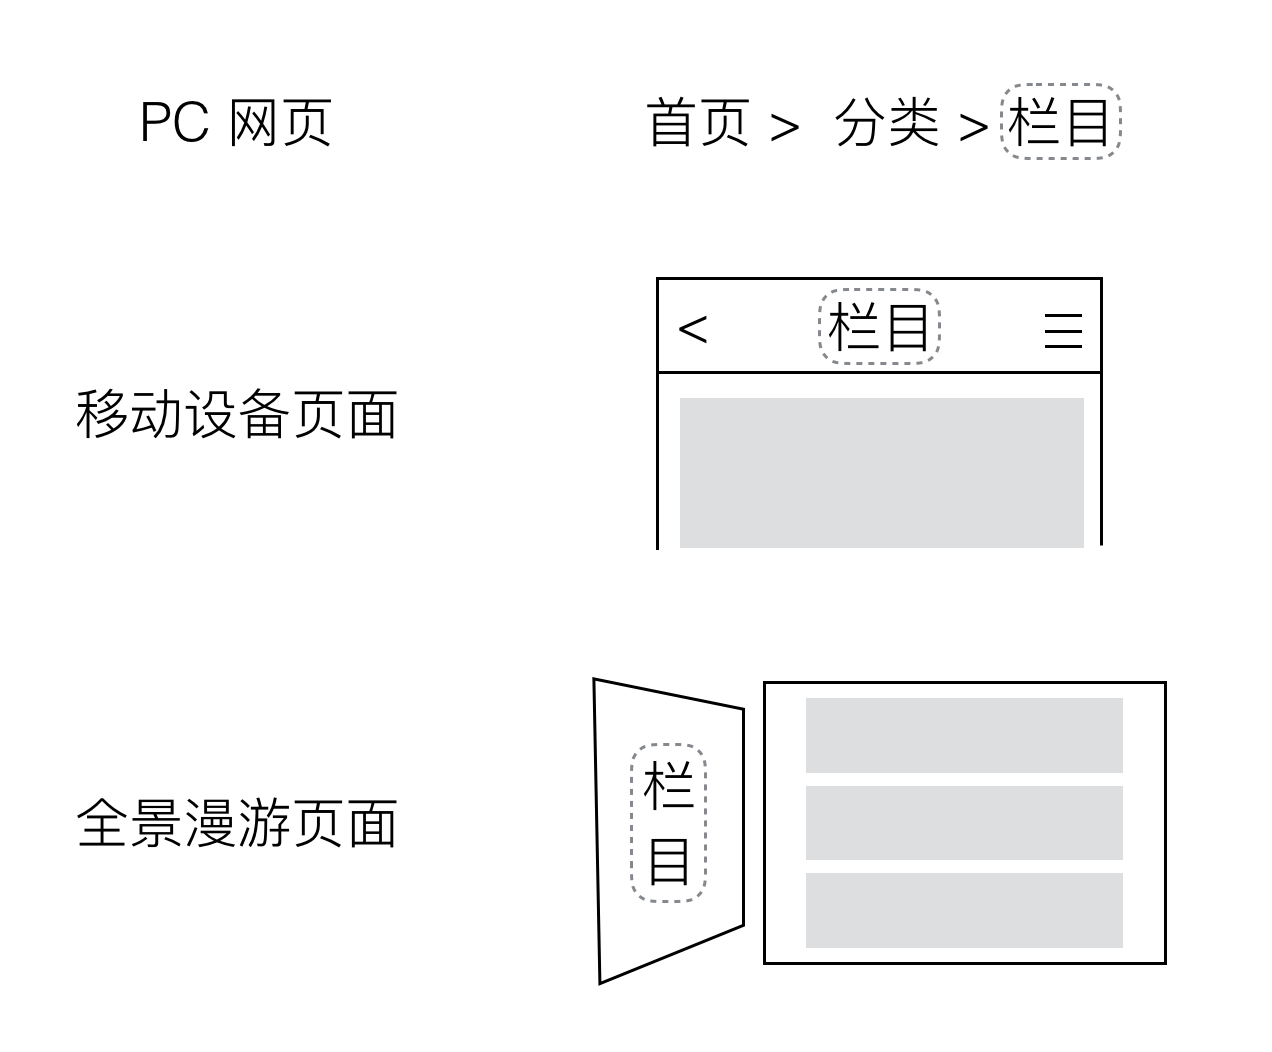
\includegraphics[width=.5\textwidth]{tab}
}
\caption{不同设备状态下的页面语境标示}
\label{fig:tab}
\end{figure}

在全景漫游的界面设计中,应当尤其注意语境的建立,以帮助用户更清晰地认知自身在导航功能中的位置,同时建立起对上下文环境的基本感知。

\subsection{增强信息}
在单个页面里尽可能多地铺陈相关信息,包括其他相关内容,减少用户反复查找的负担。信息的增加看似会对用户造成认知上的负担,但经过良好组织的信息是容易被用户快速接受的。增强信息的本质是还原给用户真实且有效的足量信息,但信息的形式应易于用户识别。研究显示,在理解复杂概念时,人对图像(尤其是图形)信息的理解准确度和速度相比理解文本信息均有一定程度的提高。而对同为文本信息的内容而言,人对数字这类表义性单一的文字识别能力也高于对其他语言的识别。故可以假设信息易识别性公式 \ref{eq:recognize}。

\begin{equation}
Icon > Graph > Number > Character 
\label{eq:recognize}
\end{equation}

根据上述内容可知,增强信息的重点在于加强图像或数字类信息的应用。结合当前设计潮流,图像和数字的确是现代网络环境下界面设计的主要构成元素,故将其作为信息的增强和补充说明是合理的。例如,在世界自然基金会(WWF)推出的 WWF Togother 主题应用中,在展示各种动植物的项目时,以数字形式展现动植物的年均生育率、平均身高、体重,以在地球模型上标示的不同颜色区域展现动物的栖息地,甚至通过 GPS 系统向用户展示当前于该动物栖息地间的距离,使用户对该类动植物的生态状况有直观的了解。这种展示方式既能充分地向用户展示相关信息,而且可以将用户代入到场景中,引起用户感同身受的心理,加强生态保护教育的记忆。

\begin{figure}[htp]
\centering
\fbox{
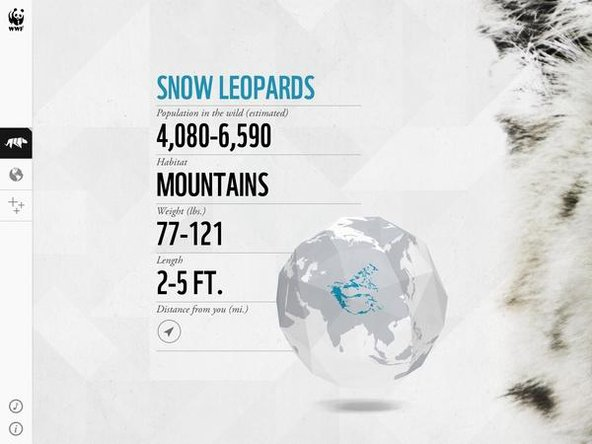
\includegraphics[width=.5\textwidth]{wwf}
}
\caption{WWF Together 主题应用截图}
\label{fig:wwf}
\end{figure}

将增强信息置于上下文语境内考量时,其应用符合人的心智模型对于信息架构的认知。从宏观角度看,用户进入应用场景时的心智模型于设计者设想的心智模型是有所冲突的,理想的应用场景应是用户一进入应用就能立即发现感兴趣的项目,但受限于现有技术能力和信息隐私的限制,用户进入场景时的心智模型是比较不符合预期的,但随着使用认知的改变而发生变化。通过信息增强令用户获得足够的有效信息,在客观上也就是使交互界面与使用者的使用习惯和 生活认知相契合,最终使用户心智模型与交互模型达到匹配\endnote{林一,陈靖,刘越,王涌天. 基于心智模型的虚拟现实与增强现实混合式移动导览系统的用户体验设计[J]. 计算机学报,2015,(02):408-422.}。

\subsection{多任务切换}
在当下计算设备的计算能力飞速提升的今天,支持多进程已是一个操作系统必备的能力,用户往往会在社交应用和工具应用中来回切换,切换任务的过程存在消耗,而这其中往往消耗掉的是用户对于当前任务状态的认知。多任务切换时保留被切换应用的状态可以帮助用户留住关于该任务的部分认知,而当用户需要切换回该任务时可以通过留存的任务状态快速回到之前工作的状态。展示多任务切换的方式有很多中,相比而言最为直观的是类似 Mac OSX 的任务窗口收缩进 Docker 栏的方式。借鉴其多任务的切换方式,可以设计全景漫游中不同场景间切换的实现方式,如图\ref{fig:multitask}所示。

\begin{figure}[htp]
\centering
\fbox{
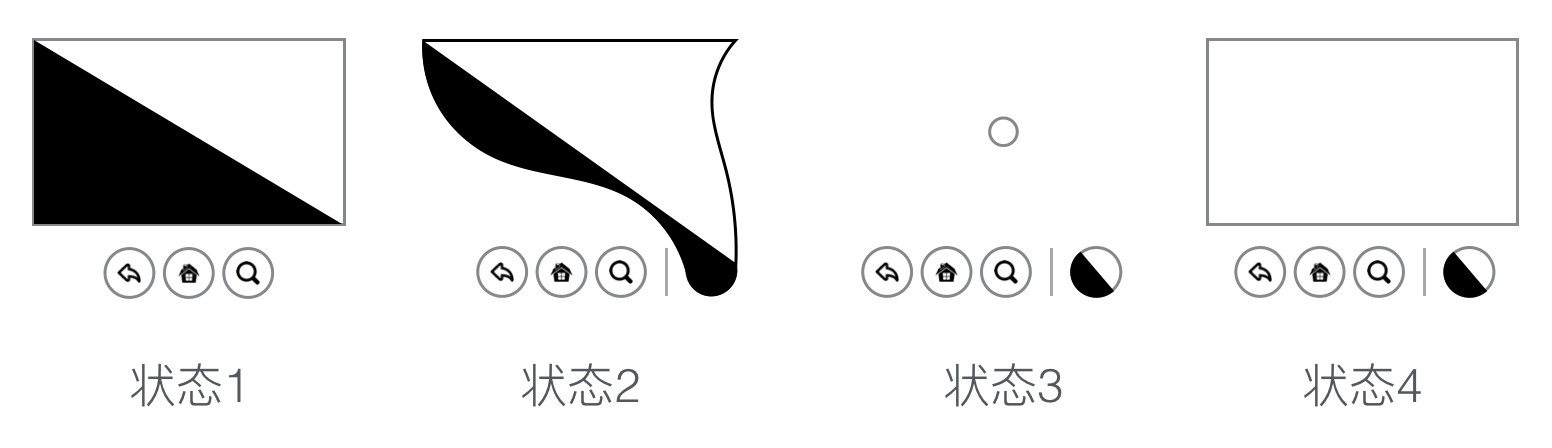
\includegraphics[width=.7\textwidth]{multitask}
}
\caption{多任务切换的交互场景}
\label{fig:multitask}
\end{figure}

上图分为四个状态
\begin{description}
	\item [状态 1] 正在使用应用 A
	\item [状态 2]用户主动打断应用运行或是用户收到系统信息而转去应用 B,此时应用 A 以 一种类似布绢收拢的形式缩小至底部全局导航栏的一侧
	\item [状态 3] 应用 A 已完全最小化到导航栏内,同时应用 B 以一个小圆点进行扩展的形式开始打开
	\item [状态 4] 应用 B 完全打开
\end{description}

此时用户能够明确地认识到应用 A 并未被关闭,同时可以通过导航栏中应用 A 的图标再次进入应用 A 并回到先前工作状态。这样就实现了用户心理上对于任务进程的闭环认识,避免用户因无法返回先前的使用状态而从头开始操作的问题。同时多任务也符合用户对于全景漫游场景应用的期望,即在一个应用中完成多种不同类型的任务,有助于提高用户的期望确认度。已有研究表明,用户的期望确认度对满意度和持续使用意愿均有显著的正向影响\endnote{代宝,刘业政. 基于期望确认模型、社会临场感和心流体验的微信用户持续使用意愿研究[J]. 现代情报,2015,(03):19-23.},故多任务切换的功能对全景漫游应用的体验起到了提升的作用。

\section{场景交互}

\subsection{直观的交互}
WYSIWYG,即“所见即所得”是一种常见的编辑模式,它便是一种很理想的设备交互模型,用户不必关注程序背后的逻辑,甚至不必关心自己编辑的文章真实存储的数据是何种形式,只需要看到屏幕上呈现的内容就是别人所能看到的内容。

全景漫游展示的正是这样一种过程,由不直观的概念转换为直观的概念。如图\ref{fig:wysiwyg}所示,人对房屋整体概念的认识观念是从具象至抽象,只有抽象简洁的概念才能方便地存储于人脑的记忆中,但涉及到具体房屋的理解时,是从单纯的“房屋”名词,到草图的展示,再到带有色彩的照片。而全景漫游要实现的是一个身临其境的房屋场景,是比照片更贴近真实房屋的信息载体。全景漫游的内容注重交互形式和体验感受的留存,不注重内容的记忆,故直观的交互符合其交互需要。

\begin{figure}[htp]
\centering
\fbox{
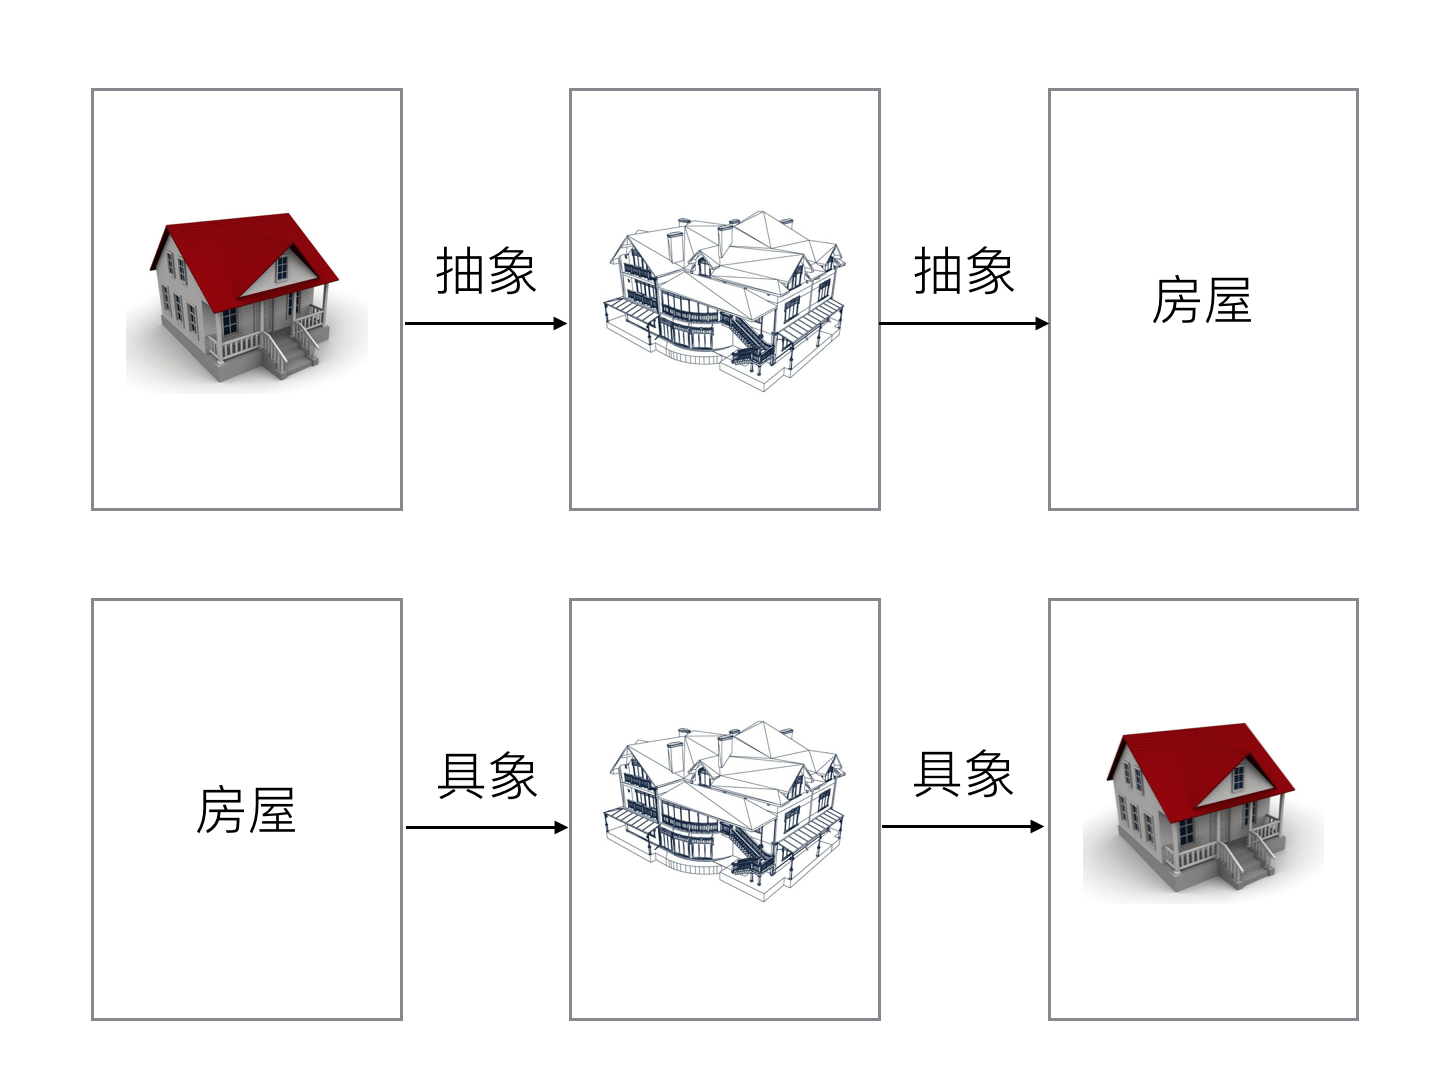
\includegraphics[width=.5\textwidth]{wysiwyg}
}
\caption{具象和抽象}
\label{fig:wysiwyg}
\end{figure}

\subsection{熟悉的定位点}
游戏中我来过的地方可以作为参照物。